%%%%%%%%%%%%%%%%%%%%%%%%%%%%%%%%%%%%%%%%%
% University/School Laboratory Report
% LaTeX Template
% Version 4.0 (March 21, 2022)
%
% This template originates from:
% https://www.LaTeXTemplates.com
%
% Authors:
% Vel (vel@latextemplates.com)
% Linux and Unix Users Group at Virginia Tech Wiki
%
% License:
% CC BY-NC-SA 4.0 (https://creativecommons.org/licenses/by-nc-sa/4.0/)
%
%%%%%%%%%%%%%%%%%%%%%%%%%%%%%%%%%%%%%%%%%

%----------------------------------------------------------------------------------------
%	PACKAGES AND DOCUMENT CONFIGURATIONS
%----------------------------------------------------------------------------------------

\documentclass[
	a4paper, % Paper size, specify a4paper (A4) or letterpaper (US letter)
	11pt, % Default font size, specify 10pt, 11pt or 12pt
]{CSUniSchoolLabReport}
\usepackage{caption, hyperref, listings, graphics, geometry}
% \addbibresource{sample.bib} % Bibliography file (located in the same folder as the template)
\geometry{left = 2.5cm, right = 2.5cm, top = 2.5cm, bottom = 2.5cm}
\renewcommand{\abstractname}{\large Abstract\\}
%----------------------------------------------------------------------------------------
%	REPORT INFORMATION
%----------------------------------------------------------------------------------------

\title{A RISC-V computer system design\thanks{\textbf{The latest version can be found at} \url{https://github.com/dream-tentacle/digital-logic-paper}}}

\author{Jun-Cheng Xiong} % Author name(s), add additional authors like: '\& James \textsc{Smith}'

\date{\today} % Date of the report

%----------------------------------------------------------------------------------------

\newdimen\Lmargin
\newdimen\Rmargin
\Lmargin=1in \advance\Lmargin by\hoffset \advance\Lmargin by\oddsidemargin
\Rmargin=\paperwidth \advance\Rmargin by-\Lmargin \advance\Rmargin by-\textwidth
\ifdim\Lmargin>\Rmargin \Rmargin=\Lmargin \fi
\def\Scentering{\leftskip=0pt plus 1fil minus \Rmargin
                \rightskip=\leftskip}

%----------------------------------------------------------------------------------------

\begin{document}

\maketitle % Insert the title, author and date using the information specified above


\begin{abstract}
    \large{
        In this project, a simple RISC-V computer system is implemented on Digilent Nexys A7-100T FPGA board. The compter system is composed of: a CPU, a data memory, an instruction memory, a vga screen, a keyboard, and a PWM audio output. The CPU is a 5-stage pipeline processor, which can execute 32-bit RISC-V instructions. The system interface is a terminal, which can execute basic commands and run two software.

        \textbf{Keywords}: RISC-V, FPGA, 5-stage pipeline, computer system
    }
\end{abstract}
\thispagestyle{empty}
\newpage

\thispagestyle{empty}
\tableofcontents
\quad
\begin{figure}[h]
    \centering
    \includegraphics[width=12cm]{image7.png}
    \caption{Digilent Nexys A7-100T FPGA board}
    \label{fig:image7}
\end{figure}


\newpage
\setcounter{page}{1}
\section{Introduction}
\subsection{Overall introduction}

In the realm of digital systems design, the creation of a fully functional computer system on a Field-Programmable Gate Array (FPGA) stands as a testament to the designer's knowledge of digital systems. This project centers around the development of a simple yet robust RISC-V computer system, implemented on the Digilent Nexys A7-100T FPGA board. At the heart of this project lies the CPU, which is a 5-stage pipeline processor that can execute 32-bit RISC-V instructions. The computer system designed for this project includes essential components such as a CPU, a data memory, an instruction memory, a VGA screen, a keyboard, and a PWM audio output. The user interacts with the system through a terminal, which supports several commands and can run two software - Snake and Piano.

This report is divided into two parts. The first segment delves into the hardware design, concentrating on the intricacies of the 5-stage pipeline CPU, memory management, and all other devices. The second part shifts focus to the software design, encompassing the implementation of the terminal, the engaging Snake game, and the musical pursuit in the form of the Piano game.

\subsection{FPGA}
The FPGA board for this project is Digilent Nexys A7-100T, a circuit design and implementation platform for classroom use. For more information, please refer to \url{https://digilent.com/reference/programmable-logic/nexys-a7/start}.

\subsection{RISC-V}
RISC-V is an open-source instruction set architecture (ISA) based on reduced instruction set computer (RISC) principles. It is a standard ISA designed to be simple, extensible, and easy to implement. In this project, I implemented a 32-bit RISC-V CPU, which can execute all 37 base instructions. For more information about RISC-V itself, please refer to \url{https://riscv.org/}.
\section{Hardware}

\subsection{5-stage pipeline CPU}
The 5-stage pipeline divides every instruction into 5 stages, and executes them in parallel, which can greatly improve the speed of the CPU. The 5 stages are: instruction fetch (IF), instruction decode (ID), execute (EX), memory access (MEM), and write back (WB). The pipeline is shown in Figure \ref{fig:image2}.

\begin{figure}[htbp]
    \Scentering
    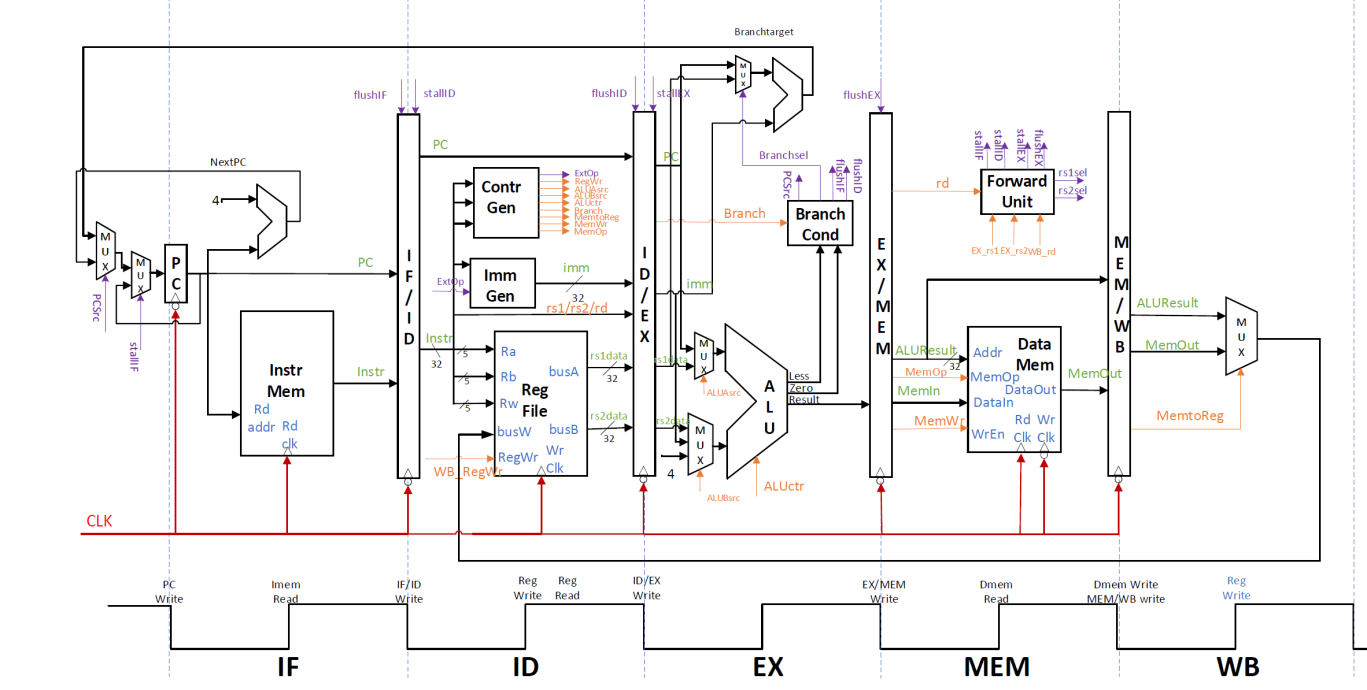
\includegraphics[width=.9\paperwidth]{image2.png}
    \caption{}
    \label{fig:image2}
\end{figure}

The cycle of clocks begins at the falling edge and ends at the next falling edge. The CPU clock is used in both the rising edge and the falling edge as follows. The regester file is written in the rising edge but read with logic assignment (thus output changes at any time). The instruction memory is read in the rising edge. The data memory (including other I/O devices) is read in the rising edge and written in the falling edge. The PC is updated in the falling edge. The pipeline registers are written and read in the falling edge.

\subsection*{Instruction fetch (IF)}
This stage fetches the instruction from the instruction memory. The PC is the program counter, which stores the address of the next instruction. Ususally, the PC is updated by adding 4 to itself, and this is calculated by a specialized add unit. At the end of the IF stage, the current PC and the instruction are stored in the pipeline register IF/ID.
\subsection*{Instruction decode (ID)}
This stage decodes the instruction and reads the register file. The register file has two read ports, which can read two registers at the same time. Other control signals are also generated in this stage. At the end of the ID stage, the PC, the regester information and the control signals are stored in the pipeline register ID/EX.

\subsection*{Execute (EX)}
This stage executes the calculation. According to the result of ALU and the control signals, a signal for branching is generated. If it is going to branch, the IF and ID stages will be flushed, and the PC will be changed. At the end of the EX stage, the PC, the result of ALU, the regester information and the control signals are stored in the pipeline register EX/MEM.

\subsection*{Memory access (MEM)}
This stage not only reads and writes the memory, but also checks if there is a hazard, which will be introduced later. At the end of the MEM stage, the PC, the result of ALU, the regester information and the control signals are stored in the pipeline register MEM/WB.

\subsection*{Write back (WB)}
This stage writes the result of ALU or the memory to the register file. Because the register file is written in the rising edge, the written value can be used in the ID stage of the same clock cycle, which is called forwarding.

\subsection*{Hazard solution}
There are three types of hazards: data hazard, control hazard and structural hazard. The structural hazard doesn't exist in this project because we don't use any hardware resource in two stages at the same time. The control hazard is solved by flushing the IF and ID stages, which we have already mentioned. The data hazard is solved by forwarding.

There are three types of data hazard: RAW (read after write), WAR (write after read) and WAW (write after write). Only the RAW appears in this design. Again, there are three types of RAW: WB-ID, WB-EX, and MEM-EX. The WB-ID is mentioned in the WB stage introduction. To solve the WB-EX hazard, we use a forwarding unit to forward the result of ALU or the memory to the EX stage. The forwarding unit checks whether one of the register data in the EX comes from the writing register. If so, the forwarding unit will change the data to the writing data. The MEM-EX hazard is also solved by the forwarding unit. The forwarding unit checks whether one of the register data in the EX comes from the writing register and the instruction is a load instruction that reads the memory and writes the register. If so, the forwarding unit will change the data to the writing data.

\subsection{Memory management}

The CPU uses byte addressing, and access all other devices through memory-mapped I/O. The memory address is 32 bits wide, and the first 12 bits are used to select the device. The address map is shown in Table \ref{tab:address-map}.
\begin{table}[h]
    \Scentering
    \begin{tabular}{|c|c|c|}
        \hline
        Address range           & Device             \\
        \hline
        0x00000000 - 0x000FFFFF & Instruction memory \\
        \hline
        0x00100000 - 0x001FFFFF & Data memory        \\
        \hline
        0x00200000 - 0x002FFFFF & VGA screen         \\
        \hline
        0x00300000, 0x00300004  & Keyboard           \\
        \hline
        0x00400000, 0x00400004  & LED                \\
        \hline
        0x00500000, 0x00500004  & timer              \\
        \hline
        0x00600000              & deprecated         \\
        \hline
        0x00700000              & deprecated         \\
        \hline
        0x00800000, 0x00800004  & PWM audio output   \\
        \hline
    \end{tabular}
    \captionof{table}{Address Map}
    \label{tab:address-map}
\end{table}

\subsection{Instruction and data memory}
The instruction and data memory are both implemented using block RAM (BRAM). The instruction memory is read-only, and the data memory is read-write. Both of them are 1MB in size. The instruction address must be aligned to 4 bytes, while the data address can be any byte address.
\subsection{VGA screen (Write-only)}
The resolution is 640x480, and the color depth is 12 bits. Because the system is totally based on a terminal and the games are using characters as the basic unit, the screen is divided into 80x30 characters of 8x16 pixels. This allows us only store 80x30 characters' ascii code.

To accelerate the screen access speed, the screen is implemented with an one-dimensional array instead of a two-dimensional array. Considering the line and column size, 11-7 bits of the address are used to represent the line number, and 6-0 bits are used to represent the column number($2^5=32,2^7=128$). The screen has a base address of 0x00200000, and is accessed with 0x00200000 + offset.
\subsection{Keyboard (Read-only)}
The input signals of the keyboard are PS2\_CLK and PS2\_DATA. With a keyboard signal processor, every byte of scan code can be generated from a stream of PS2\_DATA. The scan code is then stored in a circular buffer of 16 bytes. The buffer provides the CPU with a ``new\_key'' signal, which is high when the buffer is not empty. The CPU can read ``new\_key'' through the address 0x00300000. When the CPU reads the address 0x00300004, the buffer will pop a byte of scan code.

The driver of the keyboard is implemented in the software part. Basically, the driver is a finite state machine (Figure \ref{fig:image1}), which can be divided into 4 states: KEY\_DOWN, KEY\_UP, LONG\_KEY\_DOWN, and LONG\_KEY\_UP. The ``LONG\_'' prefix in states refers to the two-bytes scan code which mainly start with 0xE0. The break code of a key is 0xF0 succeeded by its make code, thus the KEY\_UP and LONG\_KEY\_UP states are used to detect the break code.

The driver is implemented with a C function, which has only one state change every time it is called. There are three global values, ``key\_ready'', ``two\_byte\_code'' and ``key\_up'', which are signals for applications and are set according to the state. When the state machine finds that it ends a key press, it sets ``key\_ready'' to 1, and returns (the lowest byte of) the scan code. Otherwise, it returns 0. The other two-byte scan codes are not used in this project, so we just ignore them.

\begin{figure}[!htb]
    \centering
    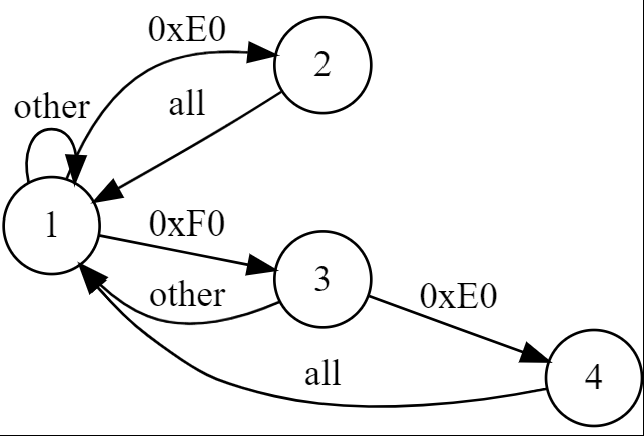
\includegraphics[width=8cm]{image1.png}
    \captionof{figure}{Keyboard driver state machine}
    \par 1: KEY\_DOWN, 2: LONG\_KEY\_DOWN, \\ 3: KEY\_UP, 4: LONG\_KEY\_UP
    \label{fig:image1}

\end{figure}

When a keycode is gotten, the software part will get the ascii code for it through an array. If the key is a signal key, it will be proceeded correspondingly.


\subsection{PWM audio output (Write-only)}
The audio pitch is based on the frequency of the PWM signal. There is a count value and a max value. Thw PWM signal is high when the count value is less than half of the max value, and low otherwise. The count value is increased by 1 every clock cycle and set back to 0 when it exceeds the max value. Thus, the pitch can be adjusted by changing the max value.

The audio has two memory addresses, 0x00800000 and 0x00800004. The first address is used to set the max value, and the second address is used to turn on/off the audio.

\subsection{Timer (Read-only)}
There are two memory addresses, 0x00500000 and 0x00500004, corresponding to the millisecond counter and the second counter. Four counters are used in the timer component: clock counter, millisecond counter 1, millisecond counter 2, and second counter. The clock frequency is 100MHz. When the clock counter reaches $10^5$, both the millisecond counters are increased by 1, and the clock counter is set back to 0. When the millisecond counter 1 reaches 1000, the second counter is increased by 1, and the millisecond counter 1 is set back to 0. The address 0x00500000 is used to read the millisecond counter 2, and the address 0x00500004 is used to read the second counter.

\section{Software}
\subsection{Terminal}
The terminal is the interface between the user and the system. The function of the terminal calls the keyboard driver function only once every time it is called. If the keyboard driver returns 0, the terminal will return immediately. Otherwise, the terminal will process the scan code and execute the corresponding command. When the system is turned on, it enters a while loop, which calls the terminal function without stopping.

The terminal has different types of responses to different key presses:
\begin{itemize}
    \item \textbf{key up}: When the global variable ``key\_up'' is set to 1, the terminal checks if the key is ``shift'', ``ctrl'', or ``alt''. If so, it sets the corresponding global flag variable to 0. Otherwise, it does nothing.
    \item \textbf{key down}: When the global variable ``key\_up'' is set to 0:
          \begin{itemize}
              \item \textbf{signal keys}: If the key is ``shift'', ``ctrl'', or ``alt'', the terminal sets the corresponding global flag variable to 1.
              \item \textbf{backspace}: If the key is ``backspace'', the terminal deletes the last character in the buffer and put a space in the screen.
              \item \textbf{enter}: If the key is ``enter'', the terminal executes the command in the buffer. If the command is not recognized, the terminal does nothing.
              \item \textbf{caps lock}: If the key is ``caps lock'', the terminal toggles the ``caps\_lock'' global flag variable.
          \end{itemize}
\end{itemize}
The terminal supports the following commands:
\begin{itemize}
    \item \textbf{help}: Print the help message.
    \item \textbf{clear}: Clear the screen.
    \item \textbf{fib n}: Print the first n Fibonacci numbers.
    \item \textbf{sort n ...}: Sort the following n numbers.
    \item \textbf{prime n}: Print all prime numbers less than n (using Euler's sieve).
    \item \textbf{snake}: Run the Snake game.
    \item \textbf{piano}: Run the Piano game.
\end{itemize}
\subsection{Snake}
The snake game looks like the classic snake game on Nokia phones. The snake can move in four directions, and it will die if it hits the wall or itself. The snake will grow longer when it eats food.

There are 3 different levels in the game. The speed of the snake increases as the level increases. When the ``snake'' command is executed in the terminal, a pop-up window will appear (Figure \ref{fig:image3}), and the player can choose the level by pressing 1, 2, or 3. The game will start after the player chooses the level. The player can press ``q'' to quit the game and return to the terminal.

\begin{figure}[!htb]
    \centering
    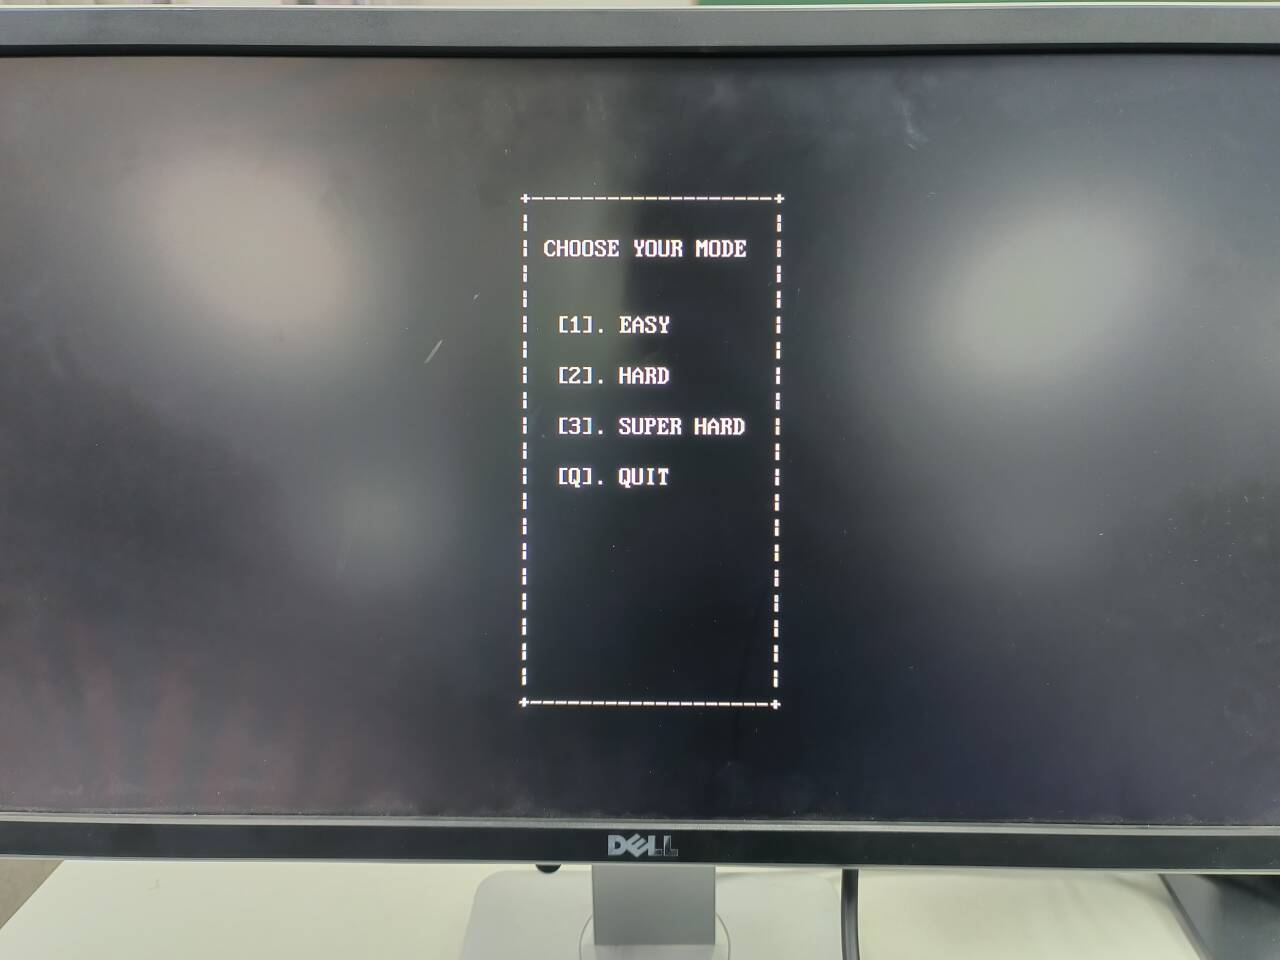
\includegraphics[width=12cm]{image3.png}
    \captionof{figure}{Snake game level selection}
    \label{fig:image3}
\end{figure}
The game looks like Figure \ref{fig:image4}. The snake is composed of squares, and the food is a circle. The score is shown in the top left corner. The player can press ``w'', ``a'', ``s'', ``d'' to control the snake. The player can press ``q'' to quit the game and return to the terminal. When the game ends, a pop-up window will appear, reads ``YOU LOSE'' in ascii art and the score (Figure \ref{fig:image5}).

\begin{figure}[!htb]
    \centering
    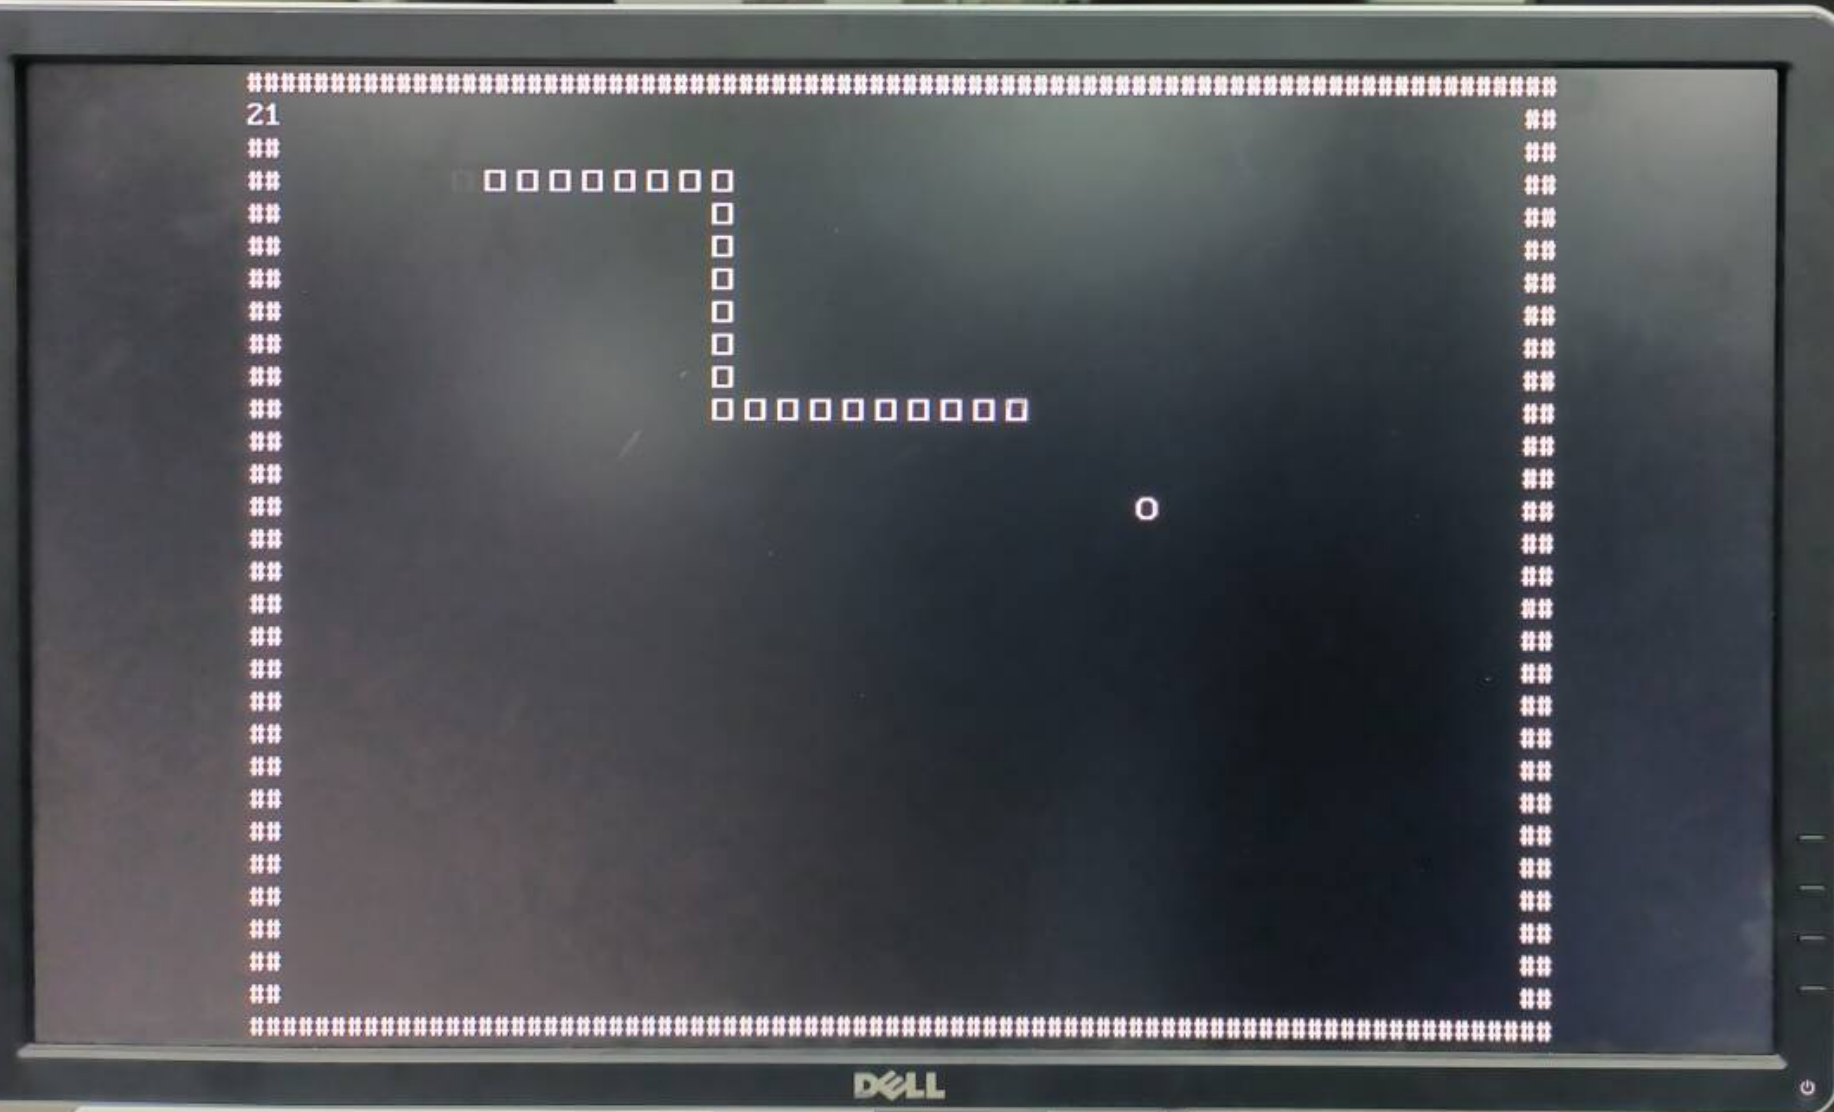
\includegraphics[width=12cm]{image4.png}
    \captionof{figure}{Snake game}
    \label{fig:image4}
\end{figure}

\begin{figure}[!htb]
    \centering
    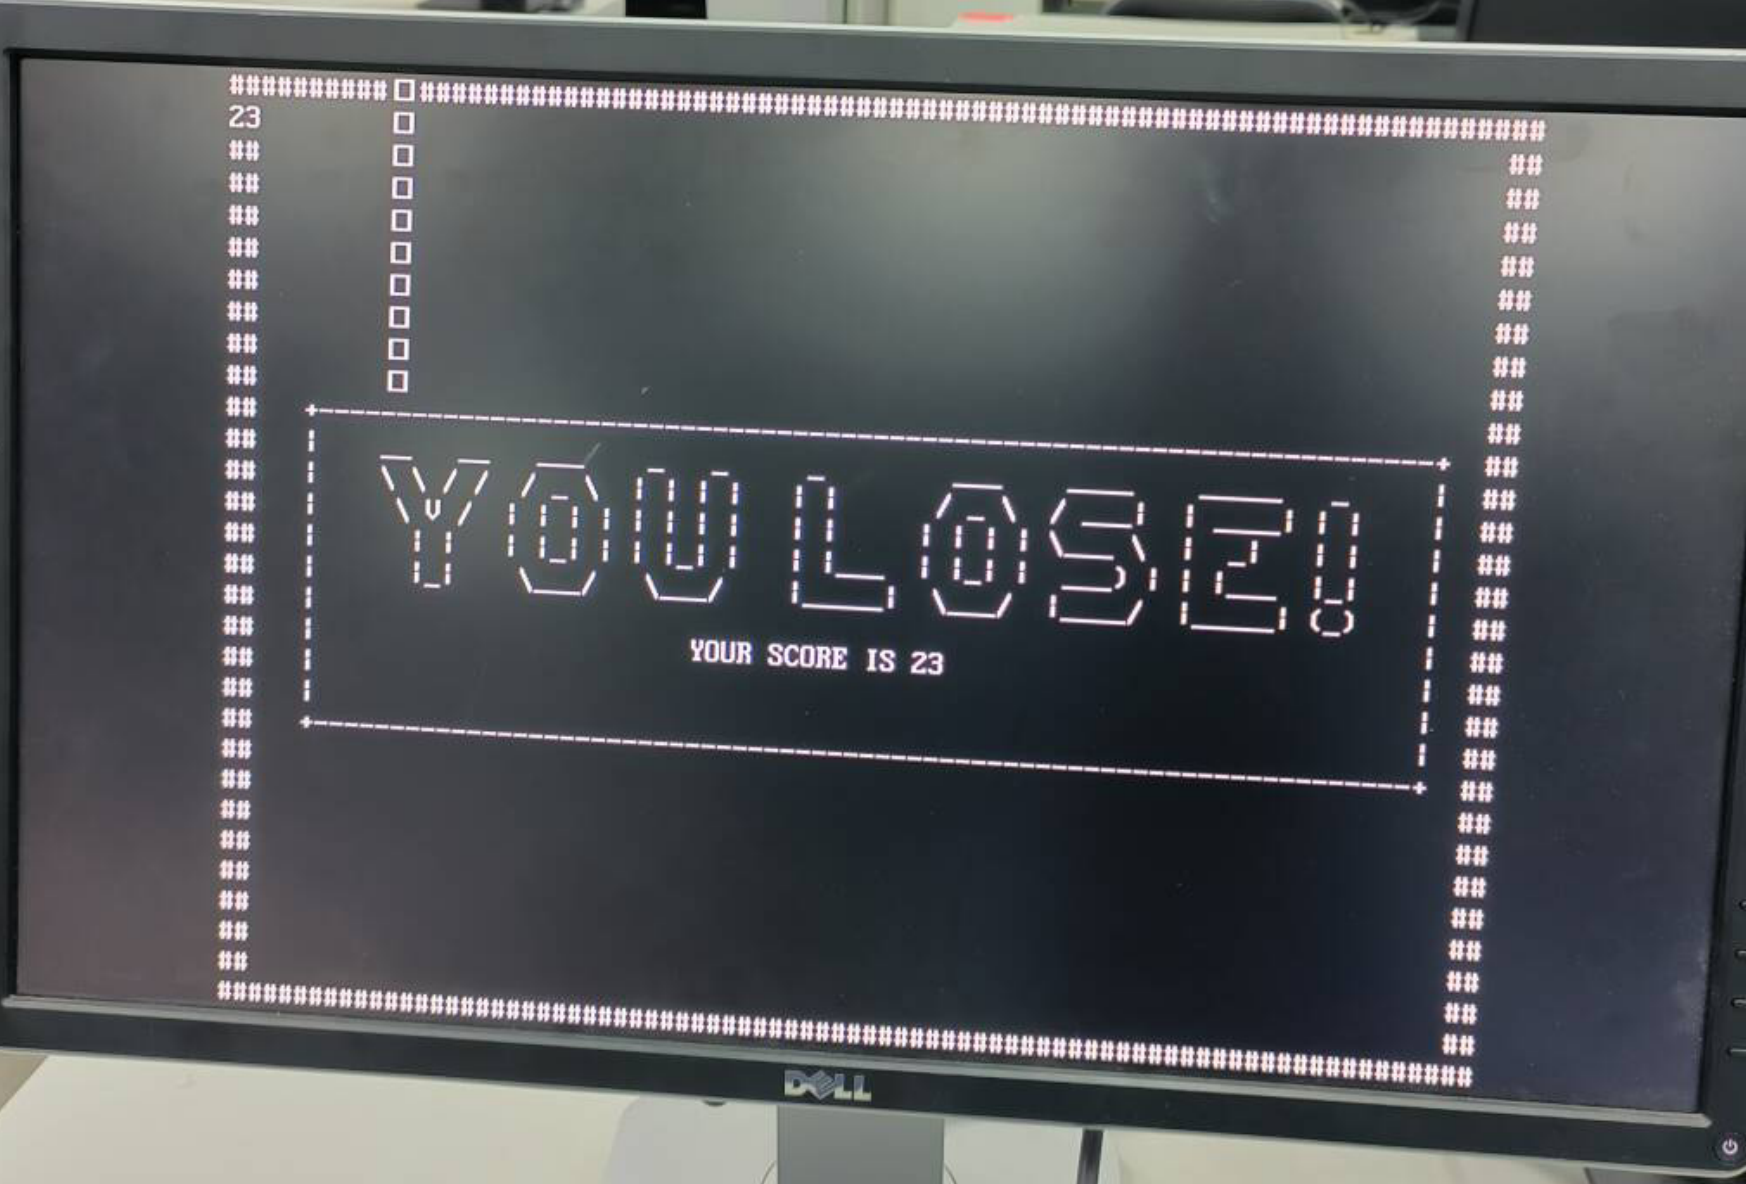
\includegraphics[width=12cm]{image5.png}
    \captionof{figure}{Snake game over}
    \label{fig:image5}
\end{figure}

\subsection{Piano}
The piano game is just a simple piano. The player can press the keys: \`, 0-9, -, = and backspace to play. The shift (ctrl) key can increase (decrease) the pitch by one octave. The player can press ``q'' to quit the game and return to the terminal.

The game looks like Figure \ref{fig:image6}. The numbers under the piano keys tell the player how to play the piano. The player can press ``q'' to quit the game and return to the terminal.

\begin{figure}[!htb]
    \centering
    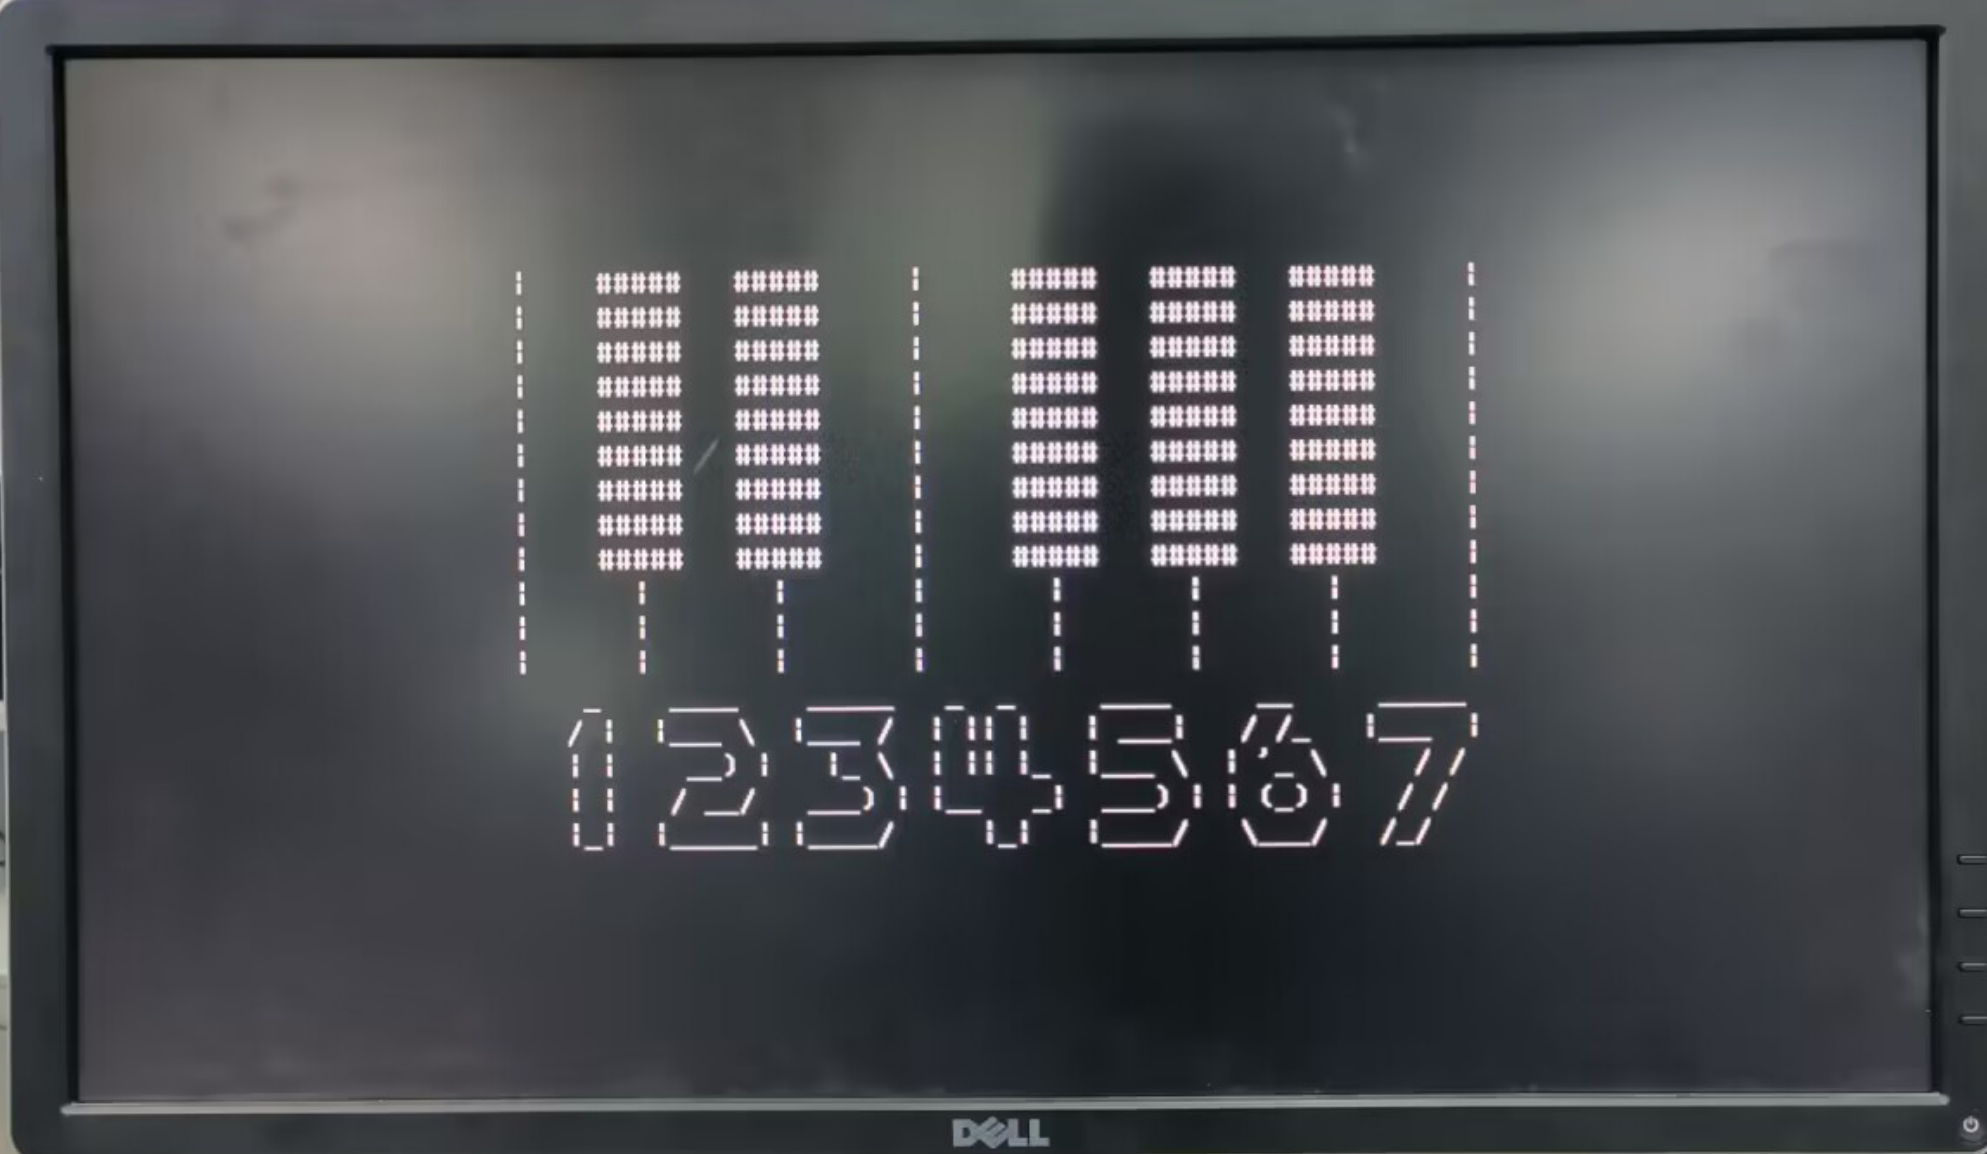
\includegraphics[width=12cm]{image6.png}
    \captionof{figure}{Piano game}
    \label{fig:image6}
\end{figure}

\end{document}